\documentclass[resume]{subfiles}


\begin{document}
\section{Introduction}
\begin{figure}[H]
\centering
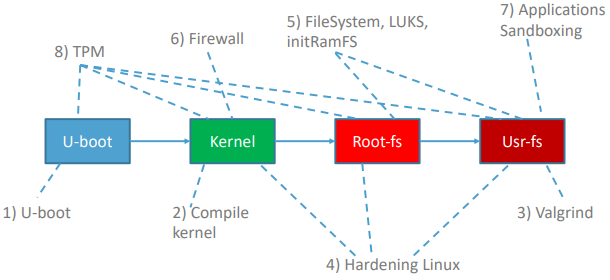
\includegraphics[width=\columnwidth]{img_0.png}
\end{figure}
\subsection{Définitions}
\begin{table}[H]
\begin{tabular}{ll}
Nom & Description\\\hline
Honeypot & "Pot de miel" ou leurre pour faire croire qu'un système non-sécurisé est présent (à tord)\\
Toolchain & Codes sources et outils nécessaires pour générer une image éxécutable (sur un système embarqué)\\
Kernel & Coeur Linux (avec le format u-boot)\\
Rootfs & Root Filesystem (avec tous les dossiers et outils utilisés par Linux)\\
Usrfs & User Filesystem (applications spécifiques à l'utilisation du système embarqué)\\
Buildroot & Ensemble de makefiles et patchs qui simplifient et automatisent la création d'un Linux pour système embarqué\\
uClibc & Librairie c de base similaire à glibc mais plus compacte (pour systèmes MMU-less)\\
Busybox & Binaire unique qui contient toutes les commandes de base (ls, cat, mv)
\end{tabular}
\end{table}
\subsection{Attaques}
\begin{enumerate}
\item Attaques de surface
\begin{enumerate}
\item Utilisateurs des ports de debug
\item Connecteurs
\item Alimentations
\end{enumerate}
\item Vecteurs d'attaque
\begin{enumerate}
\item Réseau (Ethernet, Wifi)
\item Application
\item Port série
\item USB, I2C, Flash, Bluetooth, GPS, etc...
\end{enumerate}
\end{enumerate}
\subsection{Compilation pour nanopi}
Cross-compilation (ARM) effectuée sur un système x86/x64. Buildroot est le toolchain utilisé. Les éléments suivants sont compilés :
\begin{enumerate}
\item Bootloader
\item Kernel
\item Rootfs
\end{enumerate}
Puis les images sont copiées sur la carte SD
\end{document}